\section{Principes de fonctionnement}

\vfill
\begin{itemize}
\item Sous \LaTeX, la gestion des bases de données bibliographiques se fait avec
  le système BIB\TeX. BIB\TeX\ est à la fois un format de base de données et un
  logiciel qui permet d'automatiser la mise en forme des références
  bibliographiques en interaction avec \LaTeX.
\item On utilise une base de données bibliographique (on lui donne l'extension
  \verb1.bib1 pour qu'emacs puisse automatiquement passer en mode BIB\TeX\ quand
  on l'ouvre).
\item BIB\TeX\ et \LaTeX\ pourront automatiquement insérer les appels aux
  références et formatter ces références dans la bibliographie.
\end{itemize}
\vfill

\section{Création et maintenance d'une base de données BIB\TeX}

\vfill
\begin{itemize}
\item Lorsque vous ouvrez ou créez un fichier BIB\TeX\ (avec l'extension
  \verb1.bib1), Emacs passe automatiquement en mode BIB\TeX\ ; ce qui fournit un
  certain nombre de menus spécialisés.
\item Vous entrez ensuite vos références en attribuant à chacune une catégorie
  (ouvrage, chapitre d'ouvrage, article de revue, article de conférence avec
  publication des actes, thèse de doctorat\ldots)
\item Emacs vous propose automatiquement un certain nombre de champs
  (obligatoires / facultatifs / alternatifs) à remplir.
\item Pour chaque entrée, \emph{on attribue un identifiant unique dans le
    fichier} : C'est ce qu'on appelle la \emph{clé}.
\item Elle sert à BIB\TeX/\LaTeX\ pour savoir quelle référence aller chercher,
  et elle doit être suffisament mnémotechnique pour que vous puissiez vous en
  rappeler (mais on peut aussi utiliser REF\TeX\ ! ---cf. section
  \ref{sec:reftex}).
\item Elle peut correspondre à :
  \begin{itemize}
  \item un ou des mot(s)-clé(s)
  \item un ou plusieurs noms d'auteurs
  \item exemple : \verb1chomsky.halle.SPE1
  \end{itemize}
\item Il ne peut pas y avoir d'espace entre les parties de la clé.
\end{itemize}
\vfill





\section{Ouvrage (ou Ouvrage édité)}

\vfill
\begin{verbatim}
@book{bregman.auditory,
  author = {Bregman, Albert S.},
  title = {Auditory scene analysis: The perceptual organization of
    sound},
  publisher	= {{MIT} Press},
  address = {Cambridge, MA, USA},
  year = {1990},
}
\end{verbatim}

\begin{verbatim}
@book{altmann.shillcock.cognitive,
  editor = {Altmann, Gerry T. M. and Shillcock, Richard},
  title = {Cognitive models of speech processing: The Second
    Sperlonga Meeting},
  publisher	= {Lawrence Erlbaum Associates, Inc.},
  address = {Hove, England UK},
  year = {1993},
}
\end{verbatim}
\vfill


\section{Article}

\vfill
\begin{verbatim}
@article{mcadams.segregation,
  author    = {McAdams, S.},
  title     = {Segregation of concurrent sounds. I: Effects of frequency
    modulation coherence},
  journal   = {Journal of the Acoustical Society of America},
  pages     = {2148-2159},
  year      = {1989},
  volume    = {86},
  number    = {6},
}
\end{verbatim}
\vfill


\section{Chapitre d'ouvrage}

\vfill
\begin{verbatim}
@incollection{frisch.temporally,
  author    = {Frisch, S.},
  editor    = {Broe, M. and Pierrehumbert, J. B.},
  title     = {Temporally organized lexical representations as
    phonological units},
  booktitle = {Papers in laboratory phonology V: Language acquisition and
    the lexicon},
  year      = {2002},
  publisher = {Cambridge University Press},
  address   = {Cambridge},
}
\end{verbatim}
\vfill


\section{Publication dans des actes}

\vfill
\begin{verbatim}
@inproceedings{goslin.etal.syllabification,
  author = {Goslin, J. and Content, A. and Goldman, J.-P. and Frauenfelder, U. H.},
  title = {Human and machine syllabification in French: A comparison},
  bookTitle = {II\textsuperscript{èmes} Journées d'\'Etudes Linguistiques},
  address= {Nantes, France},
  pages = {75-80},
  year = {1999},
}
\end{verbatim}
\vfill





\section{Thèse de doctorat}

\vfill
\begin{verbatim}
@phdthesis{frisch.phd,
  author = {Frisch, Stefan},
  title = {Similarity and frequency in phonology},
  school = {Northwestern University},
  type = {{PhD} Dissertation},
  year = {1996},
}
\end{verbatim}
\vfill


\section{Rapport Technique ou d'Institut}

\vfill
\begin{verbatim}
@techreport{massaro.cohen.paradigm,
  author = {Massaro, D. W. and Cohen, M. M.},
  title = {The paradigm and {FLMP} are alive and well},
  institution = {University of California},
  year = {1992},
}
\end{verbatim}
\vfill



\section{Autres types de références}
\label{sec:autres-refs}


\vfill
\begin{verbatim}
@misc{frisch.similarity,
  author = {Frisch, S. and Broe, M. and Pierrehumbert, J.},
  title = {Similarity and phonotactics in Arabic},
  year = {submitted},
}
\end{verbatim}

Un petit truc : vous pouvez remplacer \og submitted \fg par \og \verb1\submit1
\fg et introduire dans l'en-tête du document \LaTeX\ :

\begin{itemize}
\item \verb1\newcommand{\submit}{Submitted}1 ou\ldots
\item \verb1\newcommand{\submit}{Soumis}1
\end{itemize}

Pour le reste, il y a des solutions pour adapter la bibliographie à la langue
(combinaison des extensions natbib --ou jurabib-- et babelbib)

\vfill





\section{Mise en \oe{}uvre}
\label{sec:mise-en-oeuvre}

\vfill
\begin{itemize}
\item \`A l'endroit où vous citez la référence :
  \begin{itemize}
  \item \Large \verb1\cite{frisch.similarity}1
  \end{itemize}
\item \ldots et à la fin de votre document (là où vous souhaitez que la
  bibliographie apparaisse (par exemple avant les annexes) :
  \item \verb1\bibliography{nom-de-votre-base-bibtex}1
  \item \verb1\bibliographystyle{nom-du-style-de-formatage}1
\end{itemize}
\vfill

\section{Oui mais à quoi ça sert ?}
\label{sec:utilite.bibtex}


\vfill
\begin{itemize}
\item Vous ne vous préoccupez pas de la mise en page de la bibliographie ;
\item Vous ne vous préoccupez que de connaître les informations essentielles
  (noms des auteurs, année de publication, titre\ldots) ;
\item Vous laissez le logiciel se charger de la mise en page ;
\item Vous ne risquez pas de modifier votre présentation des références en cours
  de rédaction puisque vous n'êtes pas responsable de cet aspect !
\end{itemize}
\vfill





\part*{Quelques illustrations\ldots}
\label{sec:illustrations}


\section{Style \emph{plain}}
\pagecolor{\BGColorExtraLight}
\color{black}
{\large\verb1\bibliographystyle{plain}1}
\begin{center}
  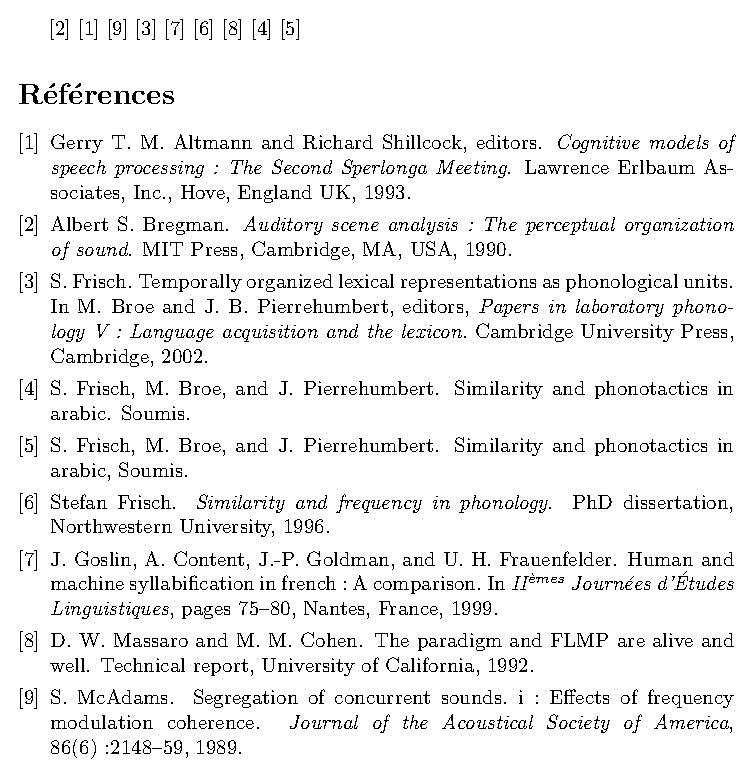
\includegraphics[width=.6\textwidth]{material/plain}
\end{center}

\section{Style \emph{unsrt}}
{\large\verb1\bibliographystyle{unsrt}1}
\begin{center}
  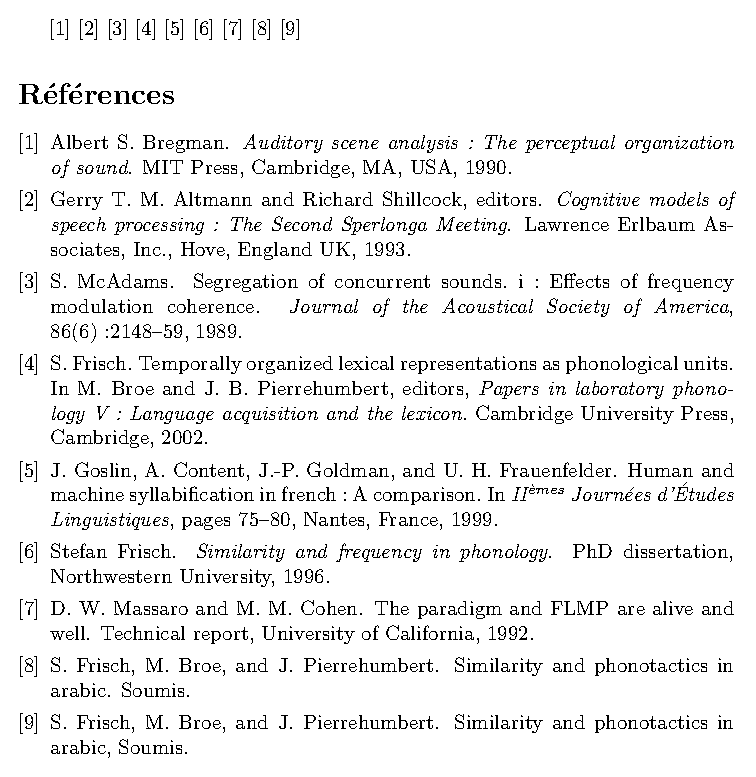
\includegraphics[width=.6\textwidth]{material/unsrt}
\end{center}

\section{Style \emph{abbrv}}
{\large\verb1\bibliographystyle{abbrv}1}
\begin{center}
  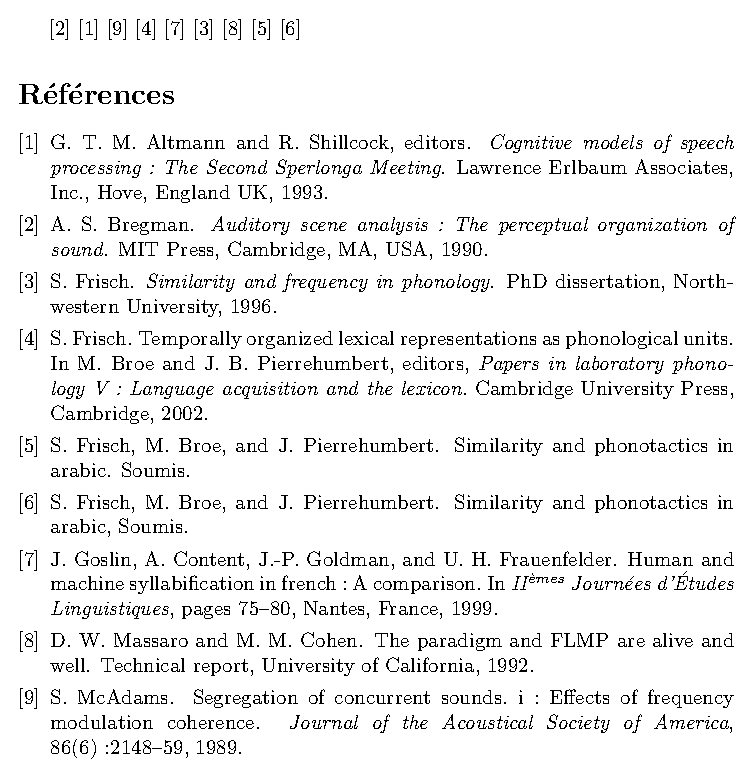
\includegraphics[width=.6\textwidth]{material/abbrv}
\end{center}

\section{Style \emph{ieeetr}}
{\large\verb1\bibliographystyle{ieeetr}1}
\begin{center}
  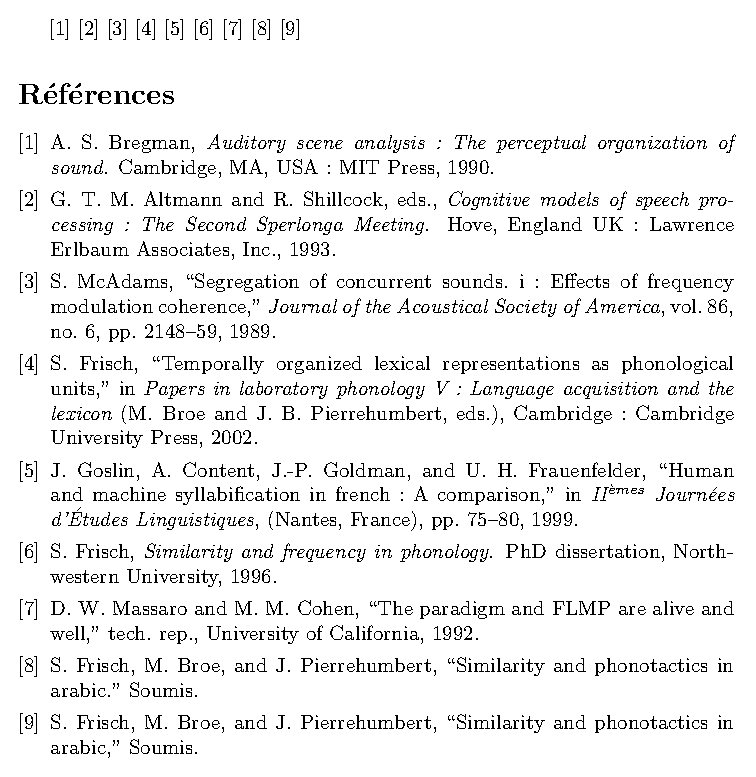
\includegraphics[width=.6\textwidth]{material/ieeetr}
\end{center}

\section{Style \emph{alpha}}
{\large\verb1\bibliographystyle{alpha}1}
\begin{center}
  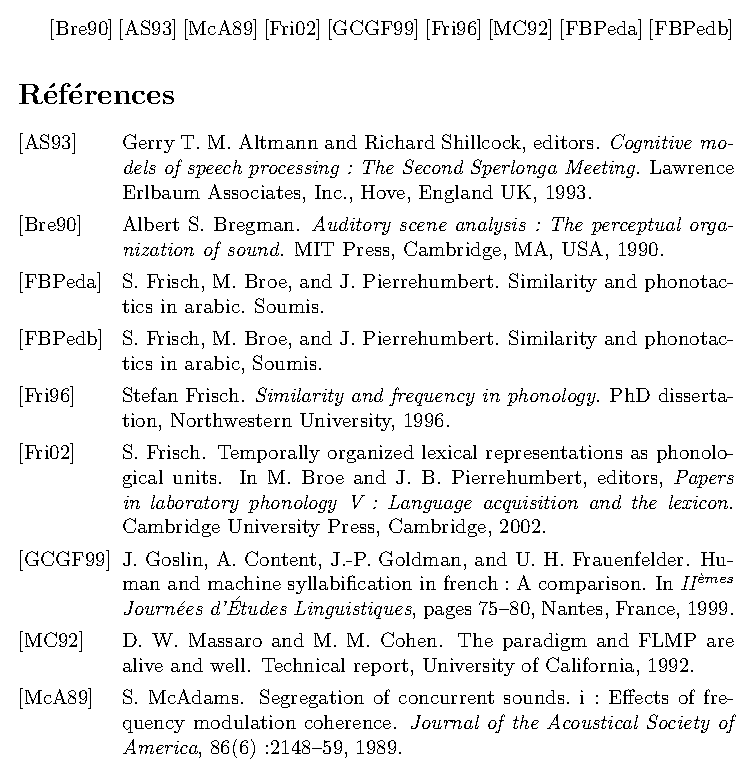
\includegraphics[width=.6\textwidth]{material/alpha}
\end{center}

\section{Style \emph{siam}}
{\large\verb1\bibliographystyle{siam}1}
\begin{center}
  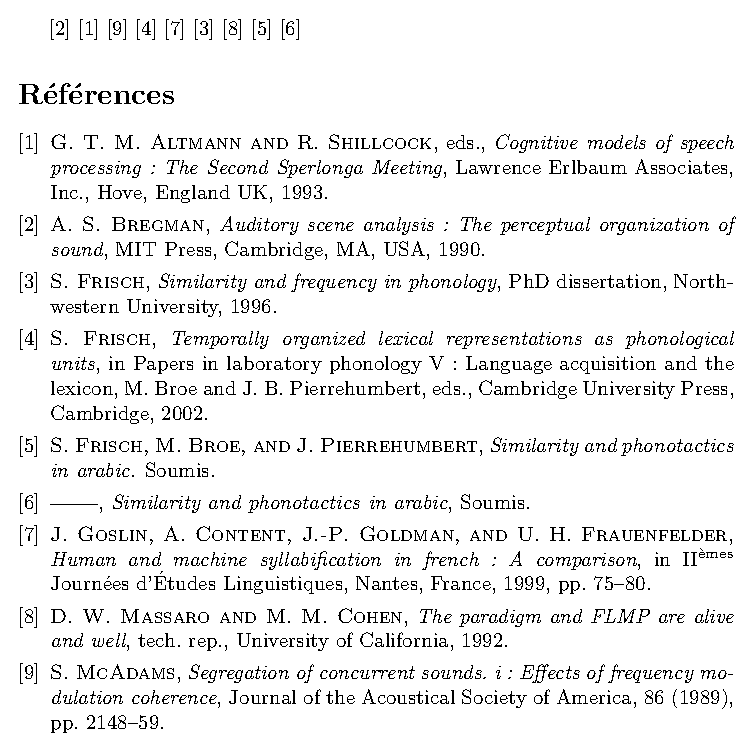
\includegraphics[width=.6\textwidth]{material/siam}
\end{center}

\section{\ldots et en utilisant l'extension \emph{natbib}}
\begin{center}
  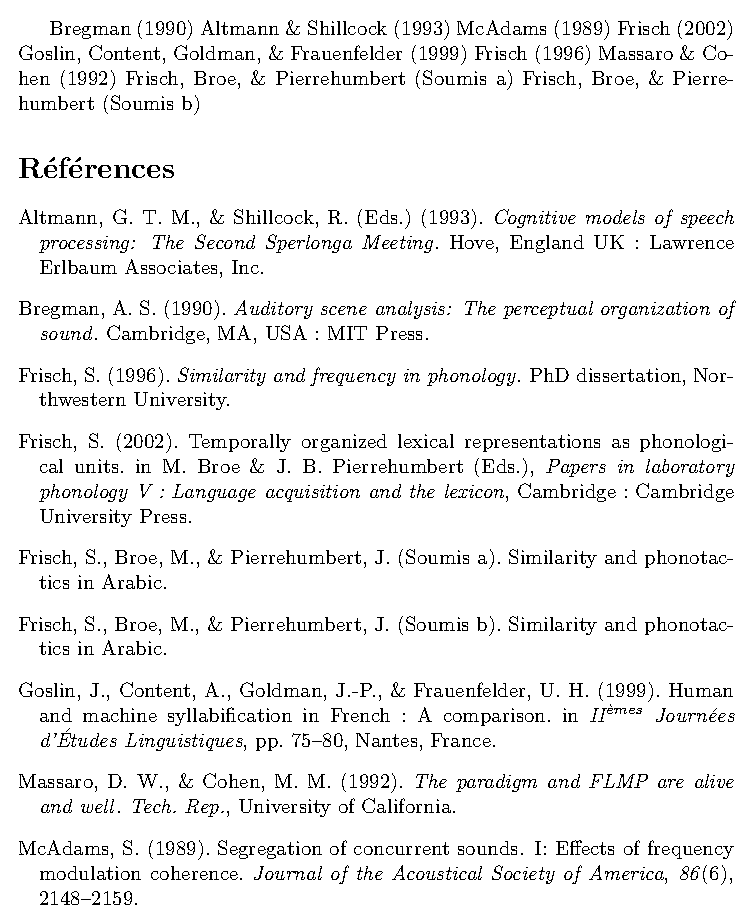
\includegraphics[width=.5\textwidth]{material/natbib-apaformat}
\end{center}





\section{Utilisation de BIB\TeX\  avec \LaTeX}
\pagecolor{\BGColor}
\color{\FGColor}

\vfill
\begin{itemize}
\item Lors de la rédaction du texte, on cite les références bibliographiques en
  désignant l'entrée correspondante dans la base de données bibliographique par
  l'instruction \verb1\cite{clé-de-la-référence}1.
\item La liste des références bibliographiques, sera construite automatiquement
  à la fin du document.
\item On utilise 2 instructions pour contrôler la gestion des références
  bibliographiques :
  \begin{itemize}
  \item \verb1\bibliography{nom-de-fichier}1 indique le nom du fichier contenant
    la base de données bibliographique.
  \item \verb1\bibliographystyle{nom-du-style}1 spécifie l'apparence des appels
    et des références. Les styles \emph{standard} sont :
    \begin{itemize}
    \item plain : [1] Noam Chomsky\ldots
    \item unsrt : idem mais dans l'ordre d'apparition des appels de citation.
    \item abbrv : [1] N. Chomsky\ldots
    \item ieetr : idem mais dans l'ordre d'apparition des appels de citation.
    \item alpha : [Cho68] Noam Chomsky\ldots
    \end{itemize}
  \end{itemize}
\end{itemize}
\vfill




\section{Compilation d'un document}
\label{sec:compilation-bibtex}


\vfill
\begin{itemize}
\item \verb1$ latex1
\item \verb1$ bibtex1
\item \verb1$ latex1
\item \verb1$ latex1
\end{itemize}
\vfill




\section{Exercices}
\label{sec:exercices}
\vfill
\begin{itemize}
\item Créez votre propre base de données bibliographique.
\item Créez un document dans lequel vous allez citer ces références en
  utilisant les techniques précédentes et en choisissant un style
  (plain, alpha, ieeetr\ldots). Nous verrons l'usage de natbib plus
  tard (c'est une extension, pas un style bibliographique).
\item Compilez votre document.
\end{itemize}
\vfill





